\begin{figure}[t]
    \centering
    \resizebox{\linewidth}{!}{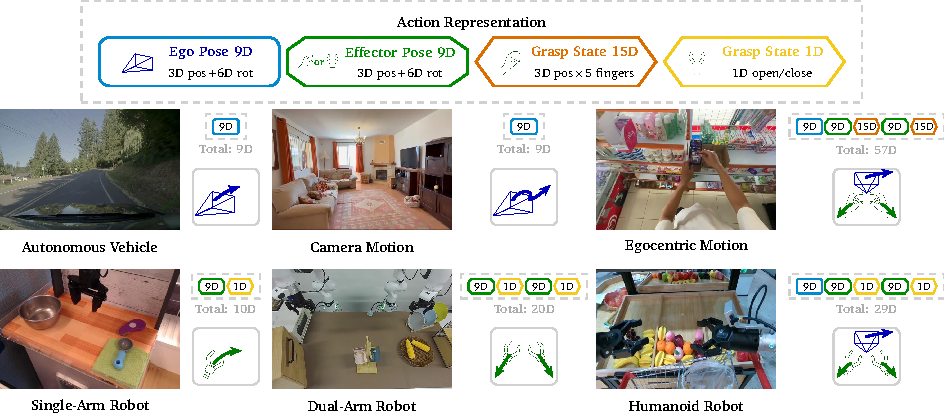
\includegraphics{figures/model_architecture/action/tikz_action_representation.pdf}}
    \caption{\textbf{Unified action representation.} We map heterogeneous embodiment controls into compact action vectors built from shared geometric components. Ego and effector motions are encoded as relative-pose pseudo-actions using 3D translation and 6D rotation (an over-parameterized rotation representation by Zhou~\citet{zhou2019continuity}, as the degree of freedom of rotation is 3), while grasp states directly encode the current manipulation state, such as fingertip positions for hands or gripper open/close values for robots. Domain-aware input and output projections handle heterogeneous action-vector lengths while preserving the shared semantic space.}
    \label{fig:action_representation}
\end{figure}
